\documentclass [a4paper] {article}

\usepackage[spanish]{babel} 
\usepackage[utf8]{inputenc} 
\usepackage{multirow} 
\usepackage{float} 

\title{R-PL6}
\author{Gabriel López Cuenca, Sergio Sanz Sacristán, Álvaro Zamorano Ortega}

\usepackage{Sweave}
\begin{document}
\Sconcordance{concordance:G16-p6.tex:G16-p6.Rnw:%
1 10 1 1 0 16 1 1 2 1 0 3 1 3 0 1 2 6 1 1 2 4 0 1 2 2 1 1 2 1 0 1 1 3 0 %
1 2 3 1 1 2 1 0 1 1 1 2 1 1 3 0 1 2 6 1 1 2 1 0 2 1 3 0 1 2 4 1 1 2 1 0 %
3 1 3 0 1 2 6 1 1 2 1 0 3 1 3 0 1 2 5 1 1 2 1 0 2 1 3 0 1 2 5 1 1 2 1 0 %
2 1 3 0 1 2 5 1 1 2 1 0 2 1 3 0 1 2 3 1}


\maketitle

\graphicspath{ {./tmp/} }

\section{Visualización en diagrama de barras.}

\subsection{Salarios medios mensuales en Europa.}
\bigskip
Hemos hecho un tratamiento de datos correspondiente a los salarios medios mensuales de los países de la Unión Europea.
Lo que buscamos es representar el conjunto de datos de estos salarios medios, para localizar, de forma clara
y sencilla la posición actual de España con respecto al resto de los países estudiados.

\bigskip
Lo primero que realizamos es importar los datos correspondientes al estudio:
\begin{Schunk}
\begin{Sinput}
> install.packages("readr")
> library("readr")
> datos <- read_csv("paises.csv")
> datos <- data.frame(datos)
\end{Sinput}
\end{Schunk}

\bigskip
Para que el diagrama quede lo más claro posible vamos a realizar un \textbf{diagrama de Pareto}. Es un tipo 
especial de gráfica de barras donde los valores graficados están organizados de mayor a 
menor. Se utiliza para para identificar los defectos que se producen con mayor frecuencia, las causas más 
comunes de los defectos o las causas más frecuentes de quejas de los clientes. Por lo tanto, ordenamos los
datos de mayor a menor haciendo uso de la función \texttt{factor.}
\begin{Schunk}
\begin{Sinput}
> datos$Pais <- factor(datos$Pais,levels=datos$Pais[order(datos$Salario)])
\end{Sinput}
\end{Schunk}

\bigskip
Para representar el diagrama utilizaremos el paquete \textbf{ggplot2}. Lo instalamos y lo cargamos.
\begin{Schunk}
\begin{Sinput}
> install.packages("ggplot2")
> library("ggplot2")
\end{Sinput}
\end{Schunk}

\bigskip
Inicializamos el diagrama e introducimos los datos. Inicialmente nos saldrán los datos en barras verticales, y
de diferentes colores al llamar a la función \texttt{geom\_bar}.
\begin{Schunk}
\begin{Sinput}
> sp <- ggplot()
> sp <- sp + geom_bar(data=datos,aes(x=datos$Pais, y=datos$Salario,
+         fill=datos$Pais), stat='identity', position='dodge',
+         show.legend=FALSE)
> source("./Funciones/diagrama.R")
> diagrama("diagrama1.png",sp)
\end{Sinput}
\end{Schunk}

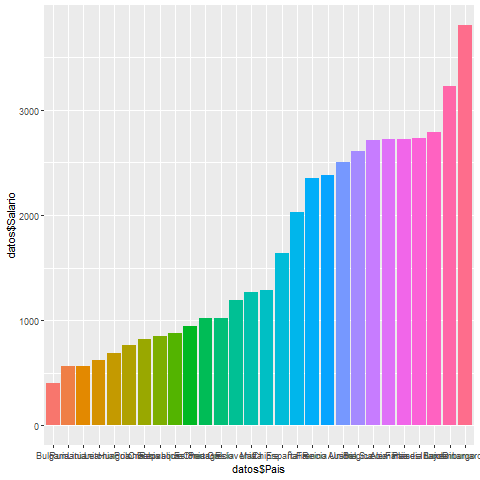
\includegraphics[width=\textwidth]{diagrama1}

\bigskip
Ya que los datos son identificados por nombre, es recomendable que estos se coloquen de la forma más visible
posible. Por lo tanto, lo que hacemos es \textbf{rotar} el diagrama para que queden los nombres en el eje y, y así
sean mucho mas visibles. Pasamos las barras de vertical a horizontal.
\begin{Schunk}
\begin{Sinput}
> sp <- sp + coord_flip()
> source("./Funciones/diagrama.R")
> diagrama("diagrama2.png",sp)
\end{Sinput}
\end{Schunk}

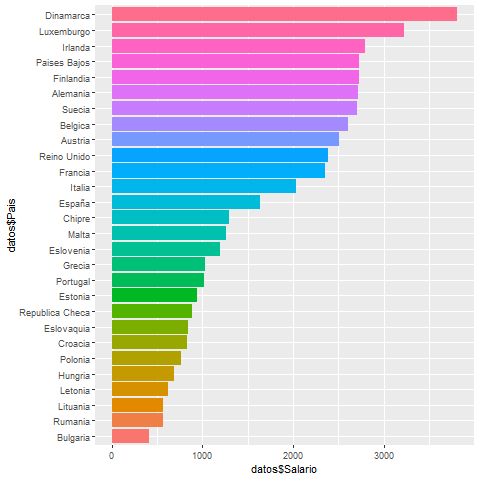
\includegraphics[width=\textwidth]{diagrama2}

\bigskip
Ahora añadimos las \textbf{etiquetas} y los \textbf{titulos} de cada uno de los ejes de nuestro diagrama y el título del mismo.
\begin{Schunk}
\begin{Sinput}
> sp <- sp + labs(x = "Paises",y="Salario")
> sp <- sp + ggtitle(label = "Salarios medios mensuales en la Unión Europea",
+         subtitle="[Datos de 2017]") + 
+         theme(plot.title = element_text(hjust = 0.5),
+         plot.subtitle = element_text(hjust = 0.5))
> source("./Funciones/diagrama.R")
> diagrama("diagrama3.png",sp)
\end{Sinput}
\end{Schunk}

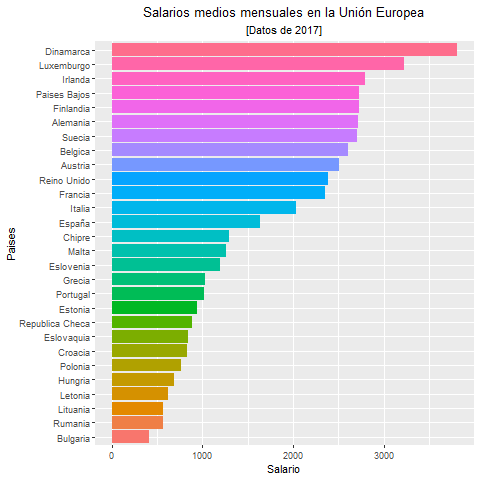
\includegraphics[width=\textwidth]{diagrama3}

\bigskip
Para que quede de una forma mucho más visual hemos decidido retirar el \textbf{fondo} gris predeterminado y ponerlo blanco.
Además \textbf{ajustamos} el eje y para que no quede espacio entre dicho eje, y las barras del diagrama usando
\texttt{scale\_y\_continuous}.
\begin{Schunk}
\begin{Sinput}
> sp <- sp + theme(panel.background = element_rect(fill = "white"))
> sp <- sp + scale_y_continuous(limits = c(0,4000) ,expand = c(0, 0))
> source("./Funciones/diagrama.R")
> diagrama("diagrama4.png",sp)
\end{Sinput}
\end{Schunk}

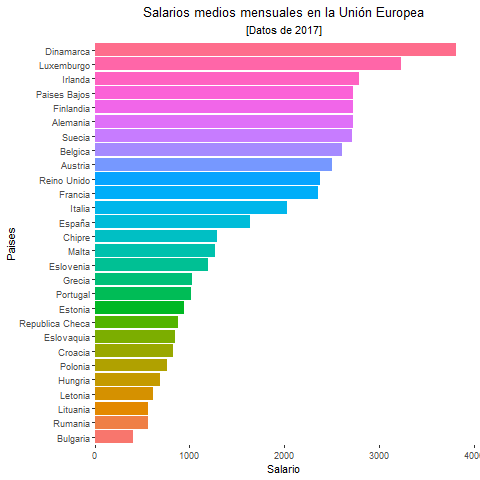
\includegraphics[width=\textwidth]{diagrama4}

\bigskip
Ahora lo que hacemos es dar el mismo \textbf{color} a todas las barras, excepto a la barra de España. Ya que nos interesa
su posición respecto al resto de países, por lo que solo destacamos esta barra.
\begin{Schunk}
\begin{Sinput}
> sp <- sp + scale_fill_manual(values = c("grey50","grey50","grey50",
+         "grey50","grey50","grey50","grey50","grey50","grey50",
+         "grey50","grey50","grey50","grey50","grey50",
+         "grey50","red","grey50","grey50","grey50","grey50",
+         "grey50","grey50","grey50","grey50","grey50","grey50",
+         "grey50","grey50"))
> source("./Funciones/diagrama.R")
> diagrama("diagrama5.png",sp)
\end{Sinput}
\end{Schunk}

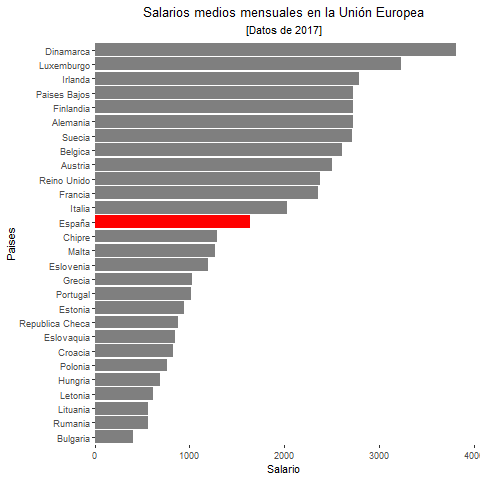
\includegraphics[width=\textwidth]{diagrama5}

\bigskip
Ahora añadimos una línea que indicará en que lugar queda la \textbf{media} de salarios medios de los paises europeos con
\texttt{geom\_hline}.
\begin{Schunk}
\begin{Sinput}
> sp <- sp + geom_hline(aes(yintercept=mean(datos$Salario)),color = "blue") + 
+         geom_text(aes(0,mean(datos$Salario),
+         label = "            Media", vjust = -1))
> source("./Funciones/diagrama.R")
> diagrama("diagrama6.png",sp)
\end{Sinput}
\end{Schunk}

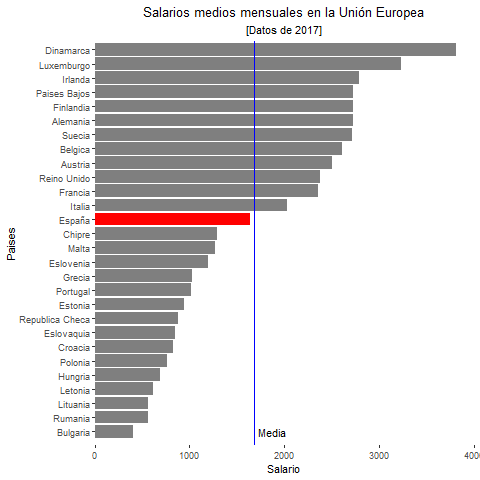
\includegraphics[width=\textwidth]{diagrama6}

\bigskip
Por último añadimos al lado de cada barra cuál es el \textbf{valor exacto} de cada dato. Así queda mucho más claro cuales
son los datos que estamos tratando, se hace con la función \texttt{geom\_text}.
\begin{Schunk}
\begin{Sinput}
> sp <- sp + geom_text(aes(datos$Pais,datos$Salario),
+         label=sprintf("           %d",datos$Salario))
> source("./Funciones/diagrama.R")
> diagrama("diagrama7.png",sp)
\end{Sinput}
\end{Schunk}

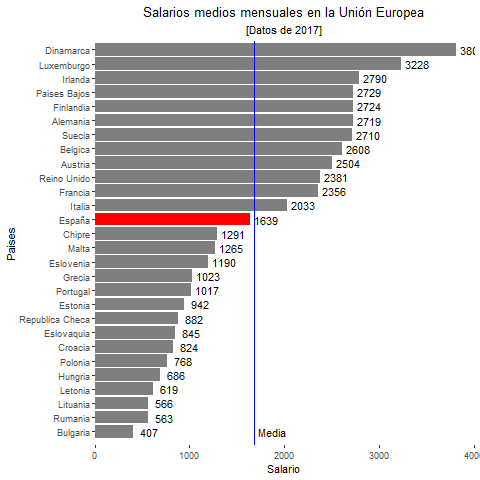
\includegraphics[width=\textwidth]{diagrama7}

\section{Visualización en mapa.}
\bigskip
Para comprender mejor la diferencia de los salarios entre los diferentes países de la Unión Europea, vamos a 
realizar una visualización en el \textbf{mapa europeo.} Para ello, utilizaremos los paquetes \texttt{ggplot2}, 
\texttt{maps}, \texttt{grid} y \texttt{rworldmap.}
\begin{Schunk}
\begin{Sinput}
> install.packages("maps")
> install.packages("rworldmap")
> library(maps)
> library(rworldmap)
\end{Sinput}
\end{Schunk}

\bigskip
En primer lugar, leeremos un \texttt{.csv} igual que el anterior pero con los nombres de los países en inglés, ya que los paquetes 
anteriores así lo necesitan.
\begin{Schunk}
\begin{Sinput}
> datos <- read_csv("countries.csv")
> datos <- data.frame(datos)
\end{Sinput}
\end{Schunk}

\bigskip
En segundo lugar se obtienen diferentes datos de \textbf{localización} a partir de las funciones antes mencionadas.
\begin{Schunk}
\begin{Sinput}
> # Obtenemos el mapa del mundo
> worldMap <- getMap()
> # Países de la Unión Europea
> europeanUnion <- datos$Pais
> # Seleccionamos los índices de los países europeos
> indEU <- which(worldMap$NAME%in%europeanUnion)
\end{Sinput}
\end{Schunk}

\bigskip
En tercer lugar, obtenemos las \textbf{coordenadas} de cada uno de los países.
\begin{Schunk}
\begin{Sinput}
> # Longitud y latitud de los bordes de los países
> europeCoords <- lapply(indEU, function(i){
+   df <- data.frame(worldMap@polygons[[i]]@Polygons[[1]]@coords)
+   df$region =as.character(worldMap$NAME[i])
+   colnames(df) <- list("long", "lat", "region")
+   return(df)
+ })
> europeCoords <- do.call("rbind", europeCoords)
\end{Sinput}
\end{Schunk}

\bigskip
En cuarto lugar, guardamos los salarios en un vector y cada uno de ellos se \textbf{relaciona} con las coordenadas
del país correspondiente.
\begin{Schunk}
\begin{Sinput}
> value <- datos$Salario
> europeanUnionTable <- data.frame(country = europeanUnion, value = value)
> europeCoords$value <- europeanUnionTable$value[match(europeCoords$region,
+         europeanUnionTable$country)]
\end{Sinput}
\end{Schunk}

\bigskip
Por último, \textbf{mostramos} por pantalla el mapa acompañado de una leyenda con la escala de salarios. A su vez,
elegimos los colores de la escala de \texttt{blanco} (salario bajo) a \texttt{negro} (salario alto) ya que se consigue
una mejor visualización que con cualquier otra escala de colores. Además, añadimos el título y eliminamos el fondo.
\begin{Schunk}
\begin{Sinput}
> P <- ggplot() + geom_polygon(data = europeCoords, aes(x = long, y = lat, 
+         group = region, fill = value),
+         colour = "black", size = 0.1) +
+         coord_map(xlim = c(-13, 35),  ylim = c(32, 71))
> P <- P + scale_fill_gradient(name = "Salario Medio", low = "#FFFFFF", 
+         high = "#000000", na.value = "grey50")
> P <- P + theme(axis.text.x = element_blank(),
+         axis.text.y = element_blank(), axis.ticks.x = element_blank(),
+         axis.ticks.y = element_blank(), axis.title = element_blank(),
+         panel.background = element_rect(fill = "white"),
+         plot.margin = unit(0 * c(-1.5, -1.5, -1.5, -1.5), "lines"))
> P <- P + ggtitle(label = "Salarios medios mensuales en la Unión Europea",
+         subtitle="[Datos de 2017]") + theme(plot.title = element_text(hjust = 0.5),
+         plot.subtitle = element_text(hjust = 0.5))
> diagrama("mapa.png",P)
\end{Sinput}
\end{Schunk}

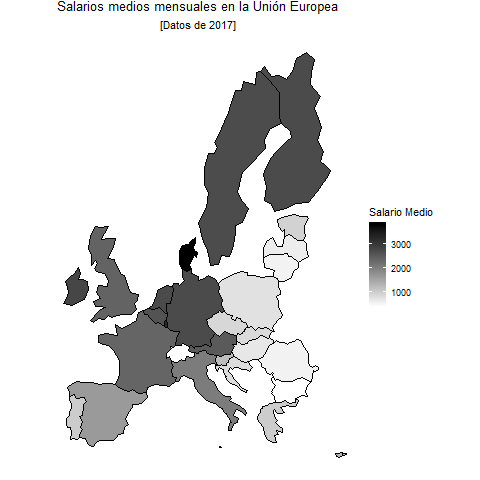
\includegraphics[width=\textwidth]{mapa}

\end{document}
